\section{Event selection} \label{sec:WBoson_Selection}


The \W boson yields are measured in the semi-muonic decay channel. The signal events, determined by the process \WToMuNu, are characterised by a high transverse momentum (\pt) muon and the presence of missing tranverse energy (\ETslash\ ), originated from the undetected neutrino. Moreover, events with similar characteristics can also be produced by other background processes, such as multi-jet events, Drell-Yan dilepton events or EWK decays. This section explain the different selections implemented to supress the background and enhance the signal.

%%------------------------------------------------------------%%
\subsection{\pPb global filter} \label{sec:WBoson_Selection_EventFilter}

In order to ensure that the samples are not contaminated by non-collision events, such as cosmics or electronic noise, a \pPb Global Event Filter (GEF) is applied. The different selections included in the \pPb GEF are described below:

\begin{itemize}
\item Primary Vertex filter: Requires a primary vertex reconstructed from at least two tracks, within a longitudinal (transverse) distance of 25~\cm (2~\cm) of the nominal interaction point.
\item HF Coincidence filter: Requires at least one tower on each side of the interaction point in the Hadron-Forward (HF) calorimeter with an energy deposit per tower of at least 3~\GeV.
\item Beam-Scraping filter: Requires at least 25$\%$ of tracks in the event to be high quality tracks.
\end{itemize}

The impact of the GEF was checked both in data and simulation. Only 0.08$\%$ of events in data and 0.06$\%$ of events in \W boson simulation, passing all the analysis cuts summarized in \sect{sec:WBoson_Selection_WSelection}, were removed by the filter.


%%------------------------------------------------------------%%
\subsection{Missing Transverse Energy} \label{sec:WBoson_Selection_MET}

Since neutrinos are not detected in the CMS detector, their presence is characterized by a particle momentum imbalance in the transverse plane, also called Missing Transverse Energy (MET). 

The MET is defined as the negative vectorial sum of the transverse momemtum of all reconstructed particles. Its coordinates along the the x and y axes in the CMS coordinate system~\cite{CMS}, can be computed as:

\begin{eqnarray*} 
\VETslash\ &=& -\sum_{particles}\ptvec \\
\ETslash\ &=& \left|\VETslash\ \right|
\end{eqnarray*}

The particle-flow algorithm (PF) \cite{PF_Reco} is used to identify the particles in the event and estimate the \ETslash\ . The PF algorithm is designed to reconstruct all stable particles such as electrons, muons, photons, charged hadrons and neutral hadrons, by taking into account all CMS sub-detectors. The outcome is an optimal determination of each particle's type, momentum and energy. This set of particles is then used to measure the \VETslash\ . The performance of the MET reconstruction in \pp data has been documented in \cite{MET_Reco,MET_PERF}.

Ideally, in an event where no neutrinos are produced, the \ETslash\ \ should be equal to zero. But since the momentum of particles is not measured with perfect precision, the sum of the reconstructed particles \ptvec does not cancel completely due to the resolution of the detector. In order to correct for the differences in the MET resolution between simulation and data, the resolution of the hadronic recoil component is smeared in the simulation to match the data as explained in \sect{sec:WBoson_Corrections_MET}.


%%------------------------------------------------------------%%
\subsection{Trigger} \label{sec:WBoson_Selection_Trigger}

The muon triggers are divided in two systems: the Level-1 (L1) trigger and the High Level Trigger (HLT). 

The L1 triggers are hardware-based and were updated during 2016 (LHC Run 2) using $\mu$TCA technology. The L1 muon trigger system is divided in 3 sub-systems: Endcap, Overlap and Barrel Muon Track Finders. The muon candidates found by each track finder are sent to the L1 Global Muon Trigger ($\mu$GMT), which process them and selects the best muon candidates. Afterwards, the L1 Global Trigger ($\mu$GT) takes the decision to either accept or reject the event based on the information provided by the $\mu$GMT and the calorimeters. In order to only consider real collisions, all \pPb L1 trigger algorithms were required to be in coincidence with a bunch crossing identified by the Beam Pick-up Timing for eXperiments (BPTX) detector. The technical information of the upgraded L1 muon trigger system is described in detail in \cite{L1_Muon_Stage2_Paper,L1_Muon_Stage2_Thesis}. 

The HLT are software-based and are only applied once an event is accepted by the L1 trigger system. The HLT muon triggers implemented for \pPb data are divided in 3 levels: the \verb#HLT_PAL1# trigger takes as input all events fired by the L1 muon trigger and does not apply any further cuts, the \verb#HLT_PAL2# trigger reconstructs the muon candidates found in the muon sub-detectors using a more sophisticated algorithm compared to L1, and the \verb#HLT_PAL3# trigger uses the muon tracks reconstructed by combining the inner tracker hits and muon tracks found by \verb#HLT_PAL2#. The HLT muon reconstruction algorithms were identical to the ones used during the 2016 \pp runs. A complete description of the CMS HLT trigger system can be found in \cite{CMS_Trigger}.

For the \W boson analysis, events that passed the muon trigger \verb#HLT_PAL3Mu12_v*# are used. This trigger requires a fully reconstructed online muon with $\pt > 12$~\GeVc. The HLT was seeded by the L1 trigger path \verb#L1_SingleMu7#, which pass events with at least one L1 muon with $\pt > 7$~\GeVc. The muon trigger was unprescaled both at L1 and HLT during the entire data taking period.

If in a given event, the main analysis trigger \verb#HLT_PAL3Mu12_v1# fired and a reconstructed muon is matched to the HLT L3 muon that fired the trigger, the reconstructed muon is considered trigger matched. The matching criteria between the reconstructed and the HLT muon is done by requiring a $\Delta{R}(\mu_{reco} , \mu_{HLT}) < 0.1$.


%%------------------------------------------------------------%%
\subsection{Muon selection} \label{sec:WBoson_Selection_MuonIdentification}

Muon candidates are identified using a tight selection optimised for muons with high \pt. The tight selection requires muon candidates to be reconstructed globally from hits in the muon stations and the tracker,  been identified with the Particle-Flow algorithm~\cite{PF_Reco} and pass the following criteria:

\begin{itemize}
\item The muon track fit has at least a $\chi^{2}$/NDF $< 10$, ensuring a reasonable fit quality.
\item The muon track has at least one hit in the muon detectors, making sure that the information from the tracker and the muon system is consistent.
\item The muon track segments are matched to at least two muon stations, making the selection consistent with the muon trigger logic.
\item The tranverse impact parameter (longitudinal distance) of the muon track is consistent with the primary vertex within 2~mm (5~mm), to reduce cosmic background and muons from decays in flight. 
\item The muon track has at least one hit in the pixel detector to further supress muons from decays in flight.
\item The muon track includes hits in at least six tracker layers to guarantee a good \pt measurement.
\end{itemize}

Apart from the muon tight selection, muon candidates are also required to be isolated in order to reduce the contribution from multi-jet background. Muons are considered isolated if the sum of the \pt of all PF particles (excluding the muon), within a cone of $\Delta{R}\left(\mu, PF\right) < 0.3$, is less than 15$\%$ of the muon \pt. The muon isolation variable is defined in \eq{eq:MuonIsolation}.

\begin{equation}
 \text{isolation} = \left(\sum_{\text{charged hadrons}}^{\text{DR}<0.3} \pt + \sum_{\text{neutral hadrons}}^{\text{DR}<0.3} \pt + \sum_{\text{photons}}^{\text{DR}<0.3} \pt\right) / \pt^\mu
 \label{eq:MuonIsolation}
\end{equation}

Since more than one muon candidate can be reconstructed in an event, the muon candidate with the highest \pt (i.e. the leading muon), is used. The event is only kept if the leading muon has a $\pt > 25$~\GeVc and $|\eta| < 2.4$. Any difference in the performance of the muon cuts observed between simulation and data, is corrected in simulation through the use of the Tag-And-Probe scale factors described in \sect{sec:WBoson_Efficiency_CorrectedEfficiency}.


%%------------------------------------------------------------%%
\subsection{Drell-Yan Veto} \label{sec:WBoson_Selection_DrellYanVeto}

A Drell-Yan veto is applied to suppress the contribution from \DYToMuMu background events. This veto removes events that contain at least two opposite sign muons with $\pt > 15$~\GeVc passing the tight muon identification and the relative muon isolation cut $iso < 0.15$, defined in \sect{sec:WBoson_Selection_MuonIdentification} .

The probability that Drell-Yan events survive the veto is checked using a Drell-Yan simulated sample. The denominator of the Drell-Yan Veto effiency is filled with the muons passing all the \W boson  analysis cuts (see \sect{sec:WBoson_Selection_WSelection}), while the numerator is filled with the same muons as long as the event pass the Drell-Yan veto. The MC survival probability is shown in \fig{fig:DrellYanVetoZEfficiency2D}.

\begin{figure}[htb]
 \begin{center}
   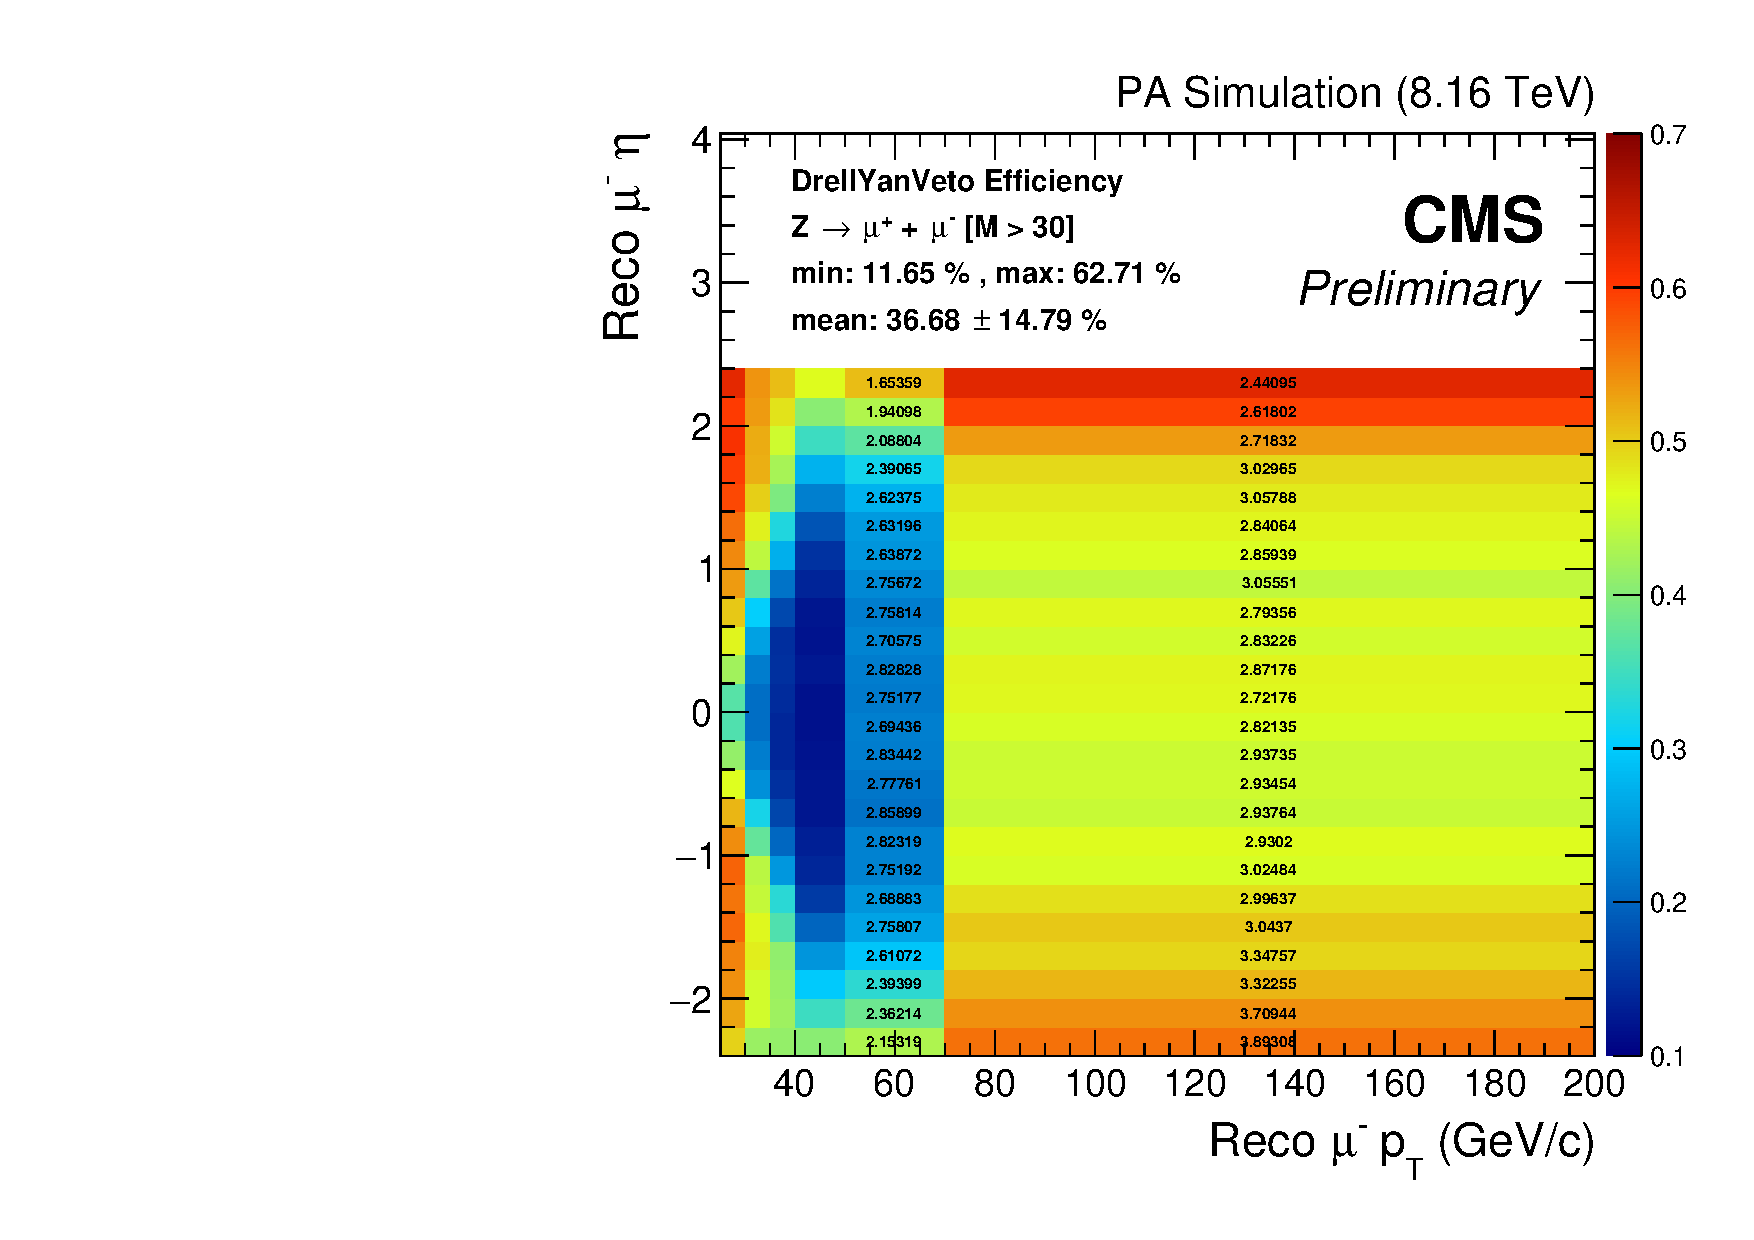
\includegraphics[width=0.45\textwidth]{Figures/WBoson/Analysis/Efficiency/Muon/PA/eff2D_Pt_Eta_MC_ZToMuMu_M_30_Inf_PA_Minus_DrellYanVeto}
   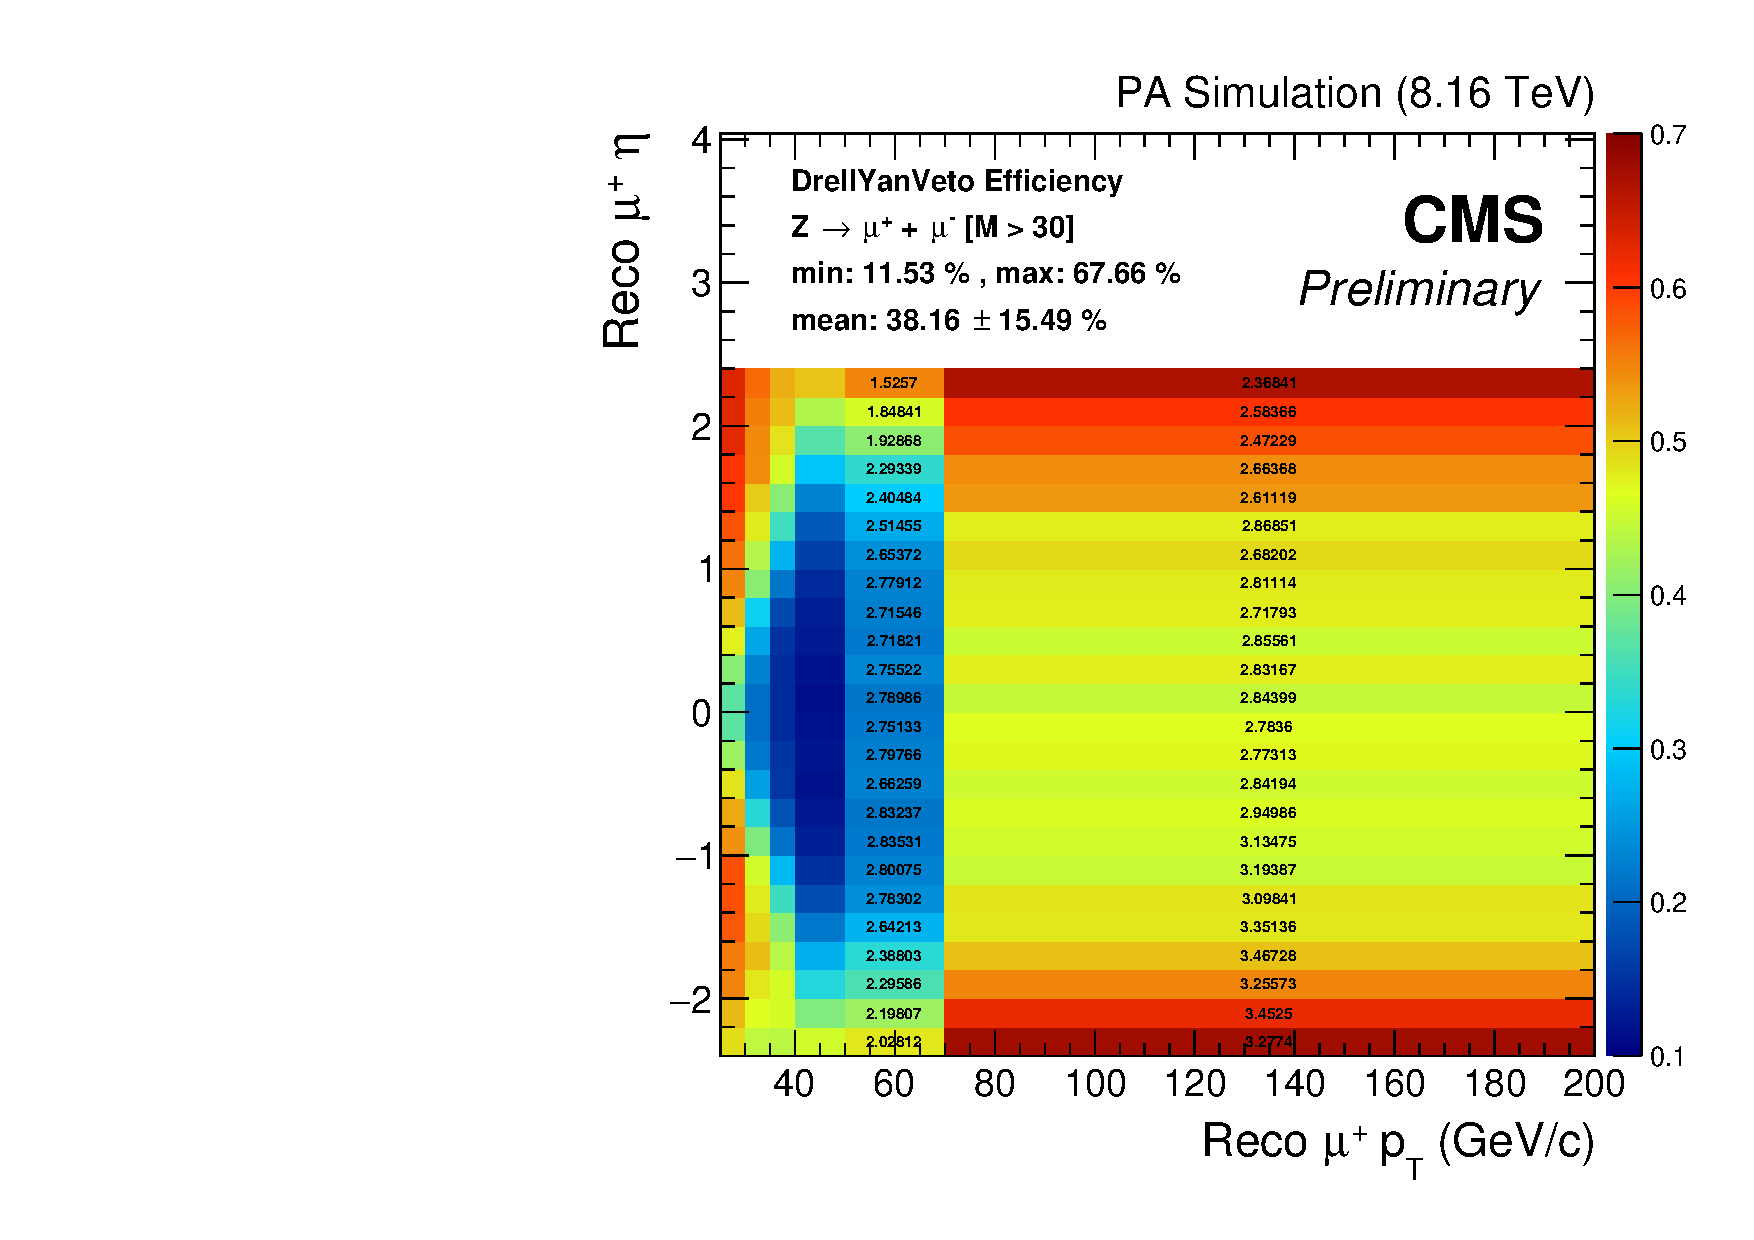
\includegraphics[width=0.45	\textwidth]{Figures/WBoson/Analysis/Efficiency/Muon/PA/eff2D_Pt_Eta_MC_ZToMuMu_M_30_Inf_PA_Plus_DrellYanVeto}
   \caption{Survival probablity of single muons from Drell-Yan ($M > 30$~\GeVcc) MC sample  as a function of the reconstructed muon $\eta$ and \pt, separated in negative (left) and positive (right) charged muons. The \pPb and \Pbp MC samples are combined as described in \sect{sec:WBoson_Sample_CombiningBeamDirection}. The relative statistical efficiency uncertainties scaled by 100 are shown for the two highest \pt bins. Reconstructed muons are required to be within $\pt > 25$~\GeVc and $|\eta| < 2.4$, be trigger matched and pass the isolation and tight selection criteria.}
   \label{fig:DrellYanVetoZEfficiency2D}
 \end{center}
\end{figure}


%%------------------------------------------------------------%%
\subsection{Summary of Event Selection} \label{sec:WBoson_Selection_WSelection}

In summary, the \W candidate selection consists of the detection of a high \pt muon, passing all identification criteria explained in \sect{sec:WBoson_Selection_MuonIdentification}. The leading muon is required to have a $\pt > 25$~\GeVc, and be trigger matched (see \sect{sec:WBoson_Selection_Trigger}). The QCD background is reduced by requiring the leading muon to be isolated. Since high \pt muons can also come from Drell-Yan or resonance decays, a dimuon veto is applied, to remove this potential source of background.

The other signature of a \W event is a high \pt neutrino, estimated through the \ETslash\ . No explicit cut is applied on \ETslash\ . The missing transverse energy is directly used to build templates and extract the yields by fitting the signal and background components. The conditions used to define the signal and background regions of interest are illustrated in \fig{fig:EventSelectionDiagram}.

\begin{figure}[htb]
 \begin{center}
   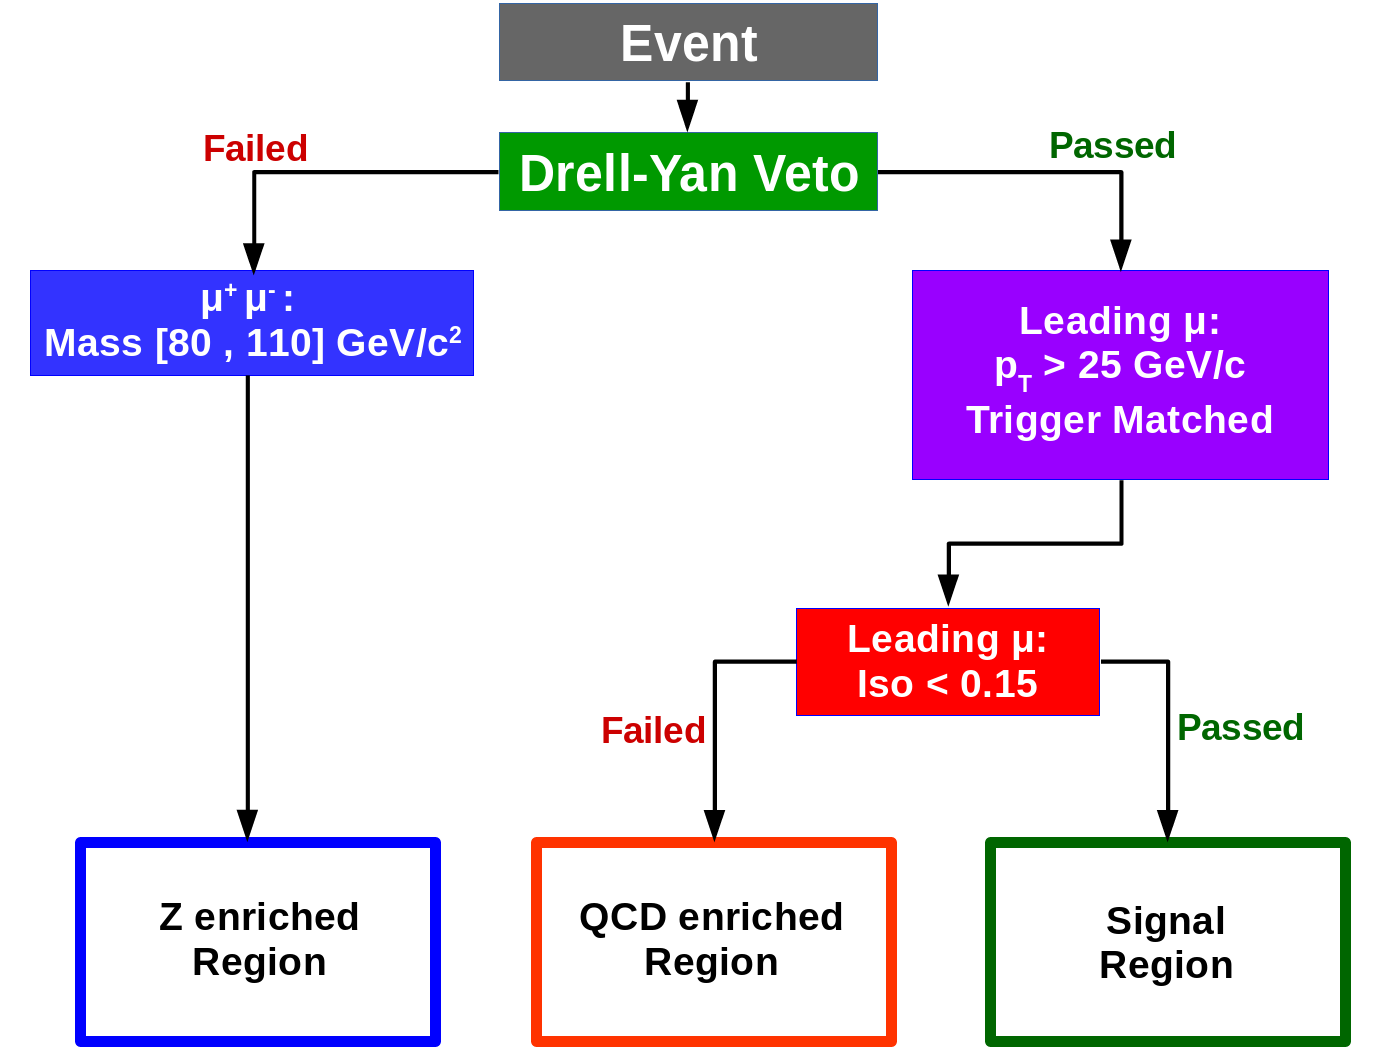
\includegraphics[width=0.9\textwidth]{Figures/WBoson/Analysis/EventSelection/FlowChar.png}
   \caption{Flowchart illustrating the way the events are classified}
   \label{fig:EventSelectionDiagram}
 \end{center}
\end{figure}


% END OF SUBSECTION
\clearpage

